\section{Performance and Discussion - N Body Problem}
\subsection{Timings}
\begin{center}
  \begin{tabular}{|c|c|c|c|}
    \hline
    Version & -OO & -O3 & -Ofast\\
    \hline
    V1 & 199.702909 & 110.818015 & 3.372535\\
    V2 & 94.216680 & 4.225227 & 4.065753\\
    V3 & 45.380386 & 3.521552 & 3.271567\\
    V4 & 24.352817 & 2.538566 & 2.454337\\
    \hline
  \end{tabular}
\end{center}
Given the optimisations described through code changes in the previous section, we have above, our timings for various optimisation flags.

Starting with Version 1, we can see that setting no optimisation flags to the code leaves us computing for a significant amount of time. this is almost halved by taking the -O3 flag. The -Ofast flag takes a significantly shorter amount of time to compute this system.

The second version of the code that we produced involved changing the way we calculated norm3. We scrapped the use of the built in pow function. This gave significant increases in time performance for the -O0 and -O3 flags, however, it actually increased computation time for the -Ofast flag. We have not understood why this is the case.

For Version 3, we altered the way in which we computed the force for each particle. Instead of calling functions for both the x and y directions, we decided to take out the elements of each equation that are the same and compute them before we computed the force in each of the $x$ and $y$ directions, thus meant that we were doing half of the original calculations. Again, this gave significant improvements in performance for -O0. Proportionately, it gave big performance improvements for -O3 and -Ofast.

The final Version took into account that we could compute the forces in half the time. This is achieved since once we know the force applied to particle $i$ from particle $j$, we know that the force applied to particle $j$ from particle $i$ is just the negative. This gave significant performance improvements with each flag.
\begin{figure}[htb]
  \begin{center}
    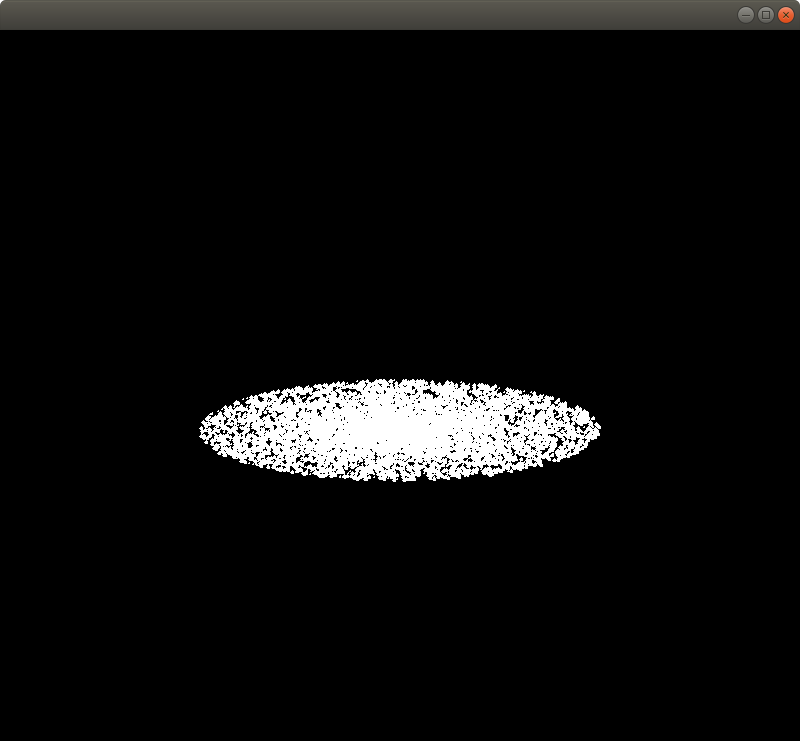
\includegraphics[width=6cm]{../images/space.jpg}
    \caption{A simulation of a galaxy}
  \end{center}
\end{figure}
\newpage
\subsection{Complexity}
Lastly, for this method, we have a plot outlining the computation times measured against $O(N^{2})$.
\begin{figure}[htb]
  \begin{center}
    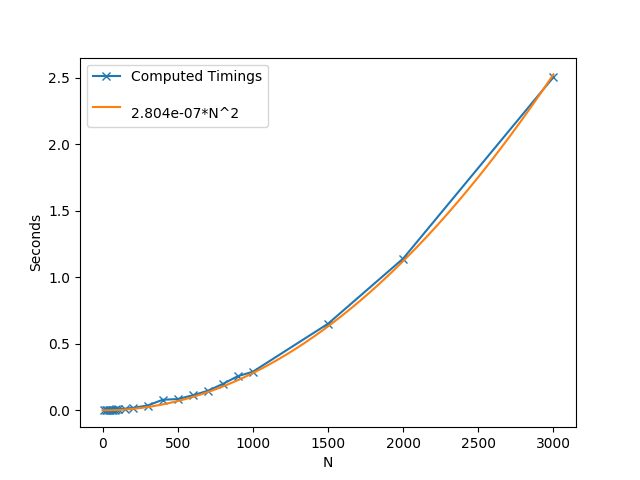
\includegraphics[width=14cm]{../images/time_complexity.png}
    \caption{Time Complexity Plot}
  \end{center}
\end{figure}
